\label{subsec:partycjonowanie}
Patrycjonowanie to proces zmiany układu partycji na dysku twardym. Jest to najważniejszy etap instalacji systemu gdyż to od niego w dużej mierze zależy jak system będzie działał. Pamiętaj, że na tym etapie pracujesz na danych zapisanych na dysku twardym. Chwila nieuwagi może spowodować utratę jego zawartości.

\subsubsection{Czysty dysk - wykorzystanie całego dostępnego miejsca}
\begin{center}
	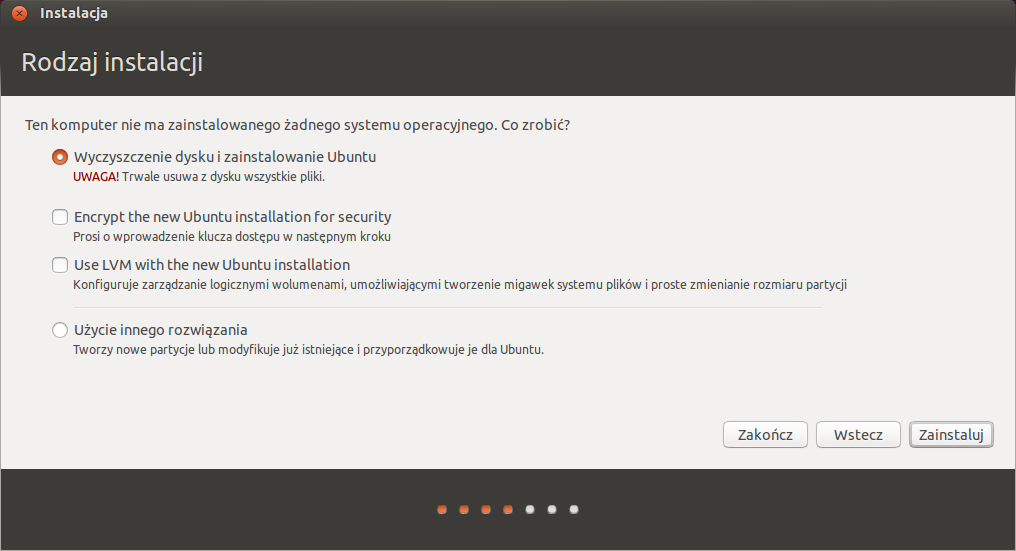
\includegraphics[scale=0.5]{images/instalator_partycjonowanie_proste.png}
\end{center}

Jeżeli na dysku twardym nie ma żadnego innego systemu operacyjnego, instalator ubuntu zaproponuje wykorzystanie całej dostępnej przestrzeni. Instalator sam dobierze odpowiedni rozmiar partycji systemowej, partycji wymiany oraz partycji użytkownika.
\begin{flushright}
Kliknij na przycisk \textbf{Zainstaluj} aby przejść dalej.\\
Zostaniesz poproszony o potwierdzenie. Upewnij się, że wszystko jest w pożądku i kliknij \textbf{Naprzód}.\\
W tym momencie wybrane zmiany zostaną zapisane na dysku twardym.
\end{flushright}
\clearpage

\subsubsection{Instalacja obok zainstalowanego Ubuntu}
\begin{center}
	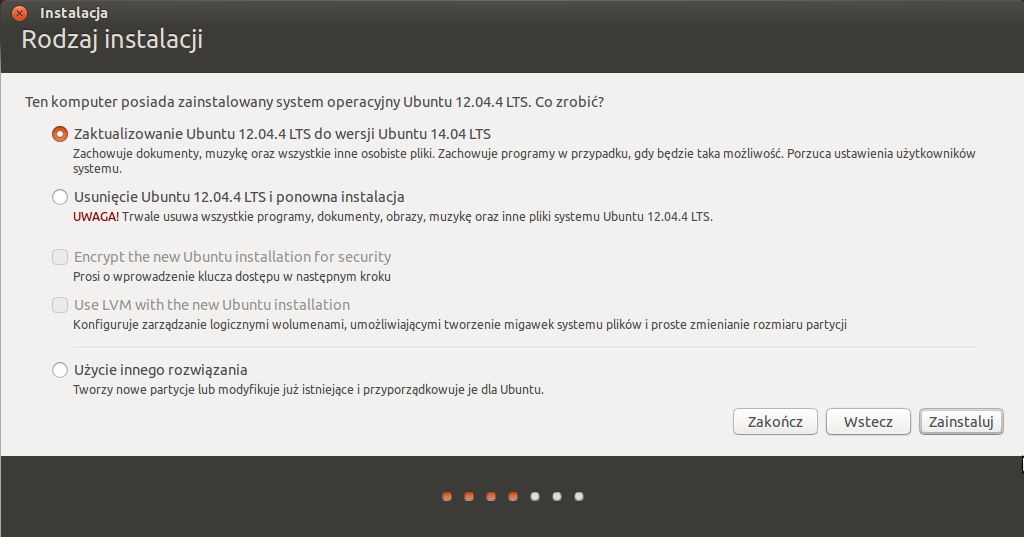
\includegraphics[scale=0.5]{images/instalator_partycjonowanie_obok_ubuntu.png}
\end{center}
Jeżeli instalator wykryje obecność wcześniej zainstalowanej innej wersji Ubuntu to zaproponuje kilka innych rozwiązań.

Po pierwsze zaproponuje aktualizację zainstalowanego systemu do najnowszego wydania. Wszystkie dane w katalogu domowym użytkownika zostaną zachowane: muzyka, filmy, dokumenty, pliki na pulpicie, osobieste ustaienia programów, zakładki i historia przeglądarki itp.
Skasowane zostaną zainstalowane w systemie programy oraz ustawienia systemowe. Instalator zaktualizuje istniejące na dysku oprogramowanie i ewentualnie pobierze aktualizacje z internetu (jeżeli wybrałeś wcześniej tą opcję).

Drugą opcją jest usunięcie zainstalowanego Ubuntu i ponowna instalacja systemu. Wszystkie dane zostaną wymazane.
\begin{flushright}
Kliknij na przycisk \textbf{Zainstaluj} aby przejść dalej.\\
Zostaniesz poproszony o potwierdzenie. Upewnij się, że wszystko jest w pożądku i kliknij \textbf{Naprzód}.\\
W tym momencie wybrane zmiany zostaną zapisane na dysku twardym.
\end{flushright}
\clearpage

\subsubsection{Instalacja obok Windowsa}
\begin{center}
	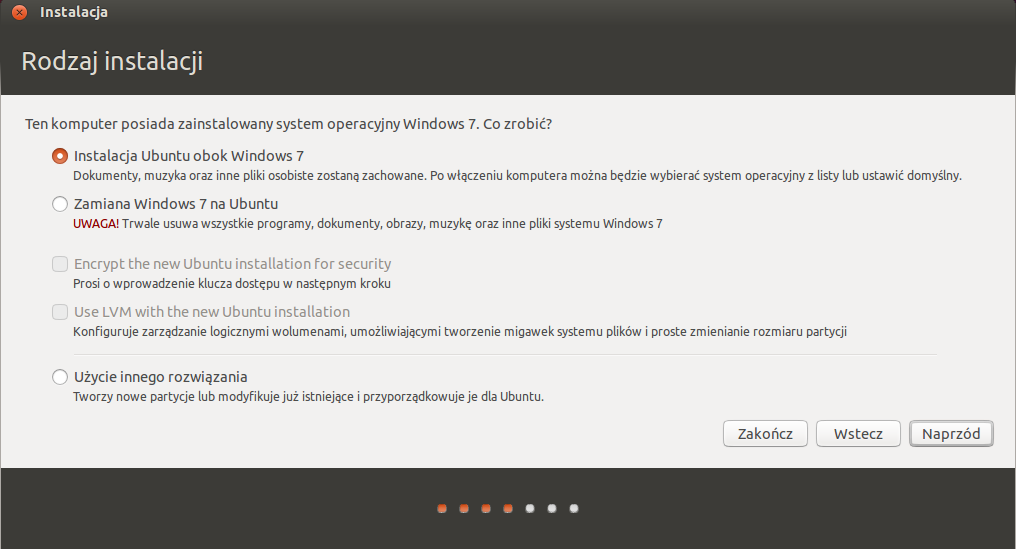
\includegraphics[scale=0.5]{images/instalator_partycjonowanie_obok_wondows7.png}
\end{center}
Jeżeli instalator wykryje obecnosć wcześniej zainstalowanego systemu Windows to zaproponuje inne rozwiązanie. Opcja "Zamiana Windows na Ubuntu" wymaże całą zawartość partycji Windows (wraz ze wszystkimi danymi) i zamiast tego zainstaluje Ubuntu. Zostało to opisane dwie strony wcześniej.
\begin{flushright}
Kliknij na przycisk \textbf{Zainstaluj} aby przejść dalej.
\end{flushright}
\clearpage
\begin{center}
	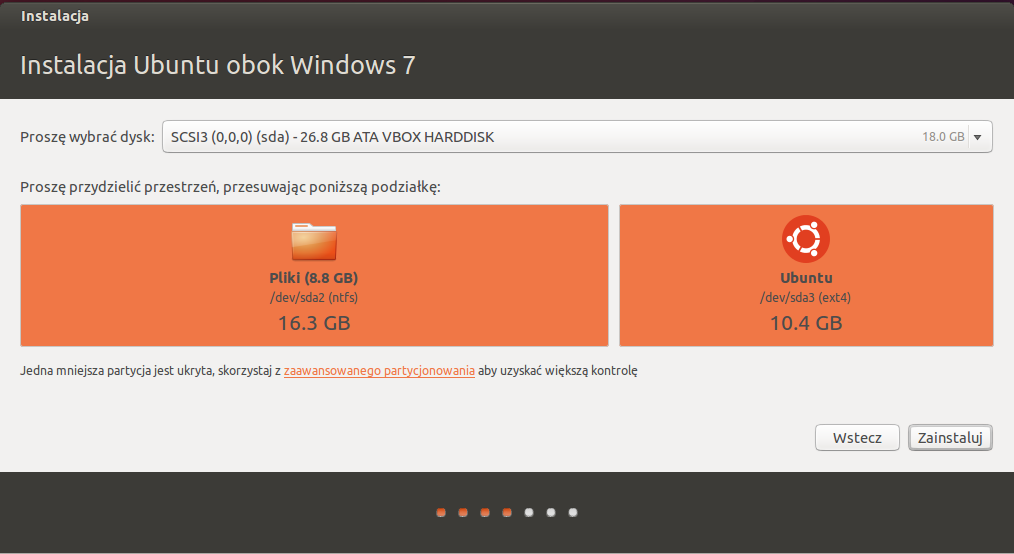
\includegraphics[scale=0.5]{images/instalator_partycjonowanie_obok_wondows7_2.png}
\end{center}
Drugą możliwością jest instalacja Ubuntu obok już zainstalowanego systemu Windows. Jeżeli wybierzesz tę opcję to następny ekran pozwoli wybrać o ile instalator ma zmniejszyć partycję na której zainstalowany jest system Windows. Użyj myszy aby przesunąć pomarańczową podziałkę w lewo (więcej miejsca dla Ubuntu) lub w prawo(więcej miejsca dla Windowsa). Oryginalna partycja systemu Windows jest oznaczona na tym obrazie jako "Pliki". Pamiętaj, że ubuntu potrzebuje minimum 6,2 gigabajta przestrzeni, ale tak mała partycja zostanie prawie w całości wypełniona przez system i na Twoje pliki pozostanie niewiele miejsca.

\begin{flushright}
Kliknij na przycisk \textbf{Zainstaluj} aby przejść dalej.\\
Zostaniesz poproszony o potwierdzenie. Upewnij się, że wszystko jest w pożądku i kliknij \textbf{Naprzód}.\\
W tym momencie wybrane zmiany zostaną zapisane na dysku twardym.
\end{flushright}
\clearpage

\subsubsection{Szyfrowanie dysku twardego}
\begin{center}
	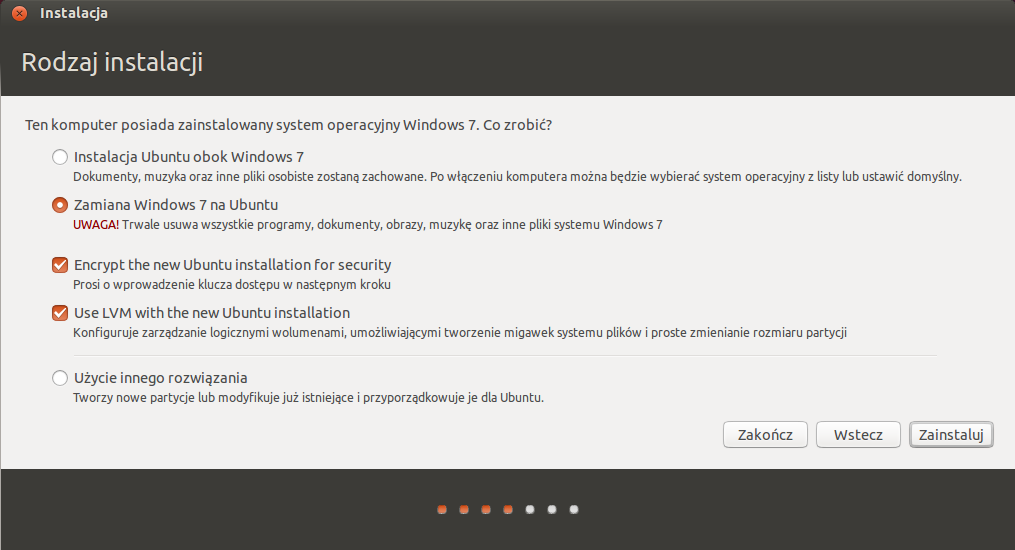
\includegraphics[scale=0.5]{images/instalator_partycjonowanie_szyfrowanie1.png}
\end{center}
Przy wyborze jednego z automatycznych rozwiązań partycjonowania miałeś możliwości zastosowania szyfrowania dysku twardego. Wybranie tej opcji ukaże ci okno jak na powyższym obrazku. Zaszyfrowanie dysku twardego sprawie, że nikt nie uzyska dostępu do twoich danych ani nie zmodyfikuje zainstalowanego systemu. Wadą tego rozwiązania jest pewien narzut na procesor komputera i związane z tym zmniejszenie płynności działania komputera. Nowoczesne procesory zapewniają akcelerację sprzętową dla obliczeń kryptograficznych, w związku z czym utrata wydajności będzie się mieścić w granicach 5\% przy intensywnych opracacjach dyskowych.
\begin{flushright}
Kliknij na przycisk \textbf{Zainstaluj} aby przejść dalej.
\end{flushright}
\clearpage
\begin{center}
	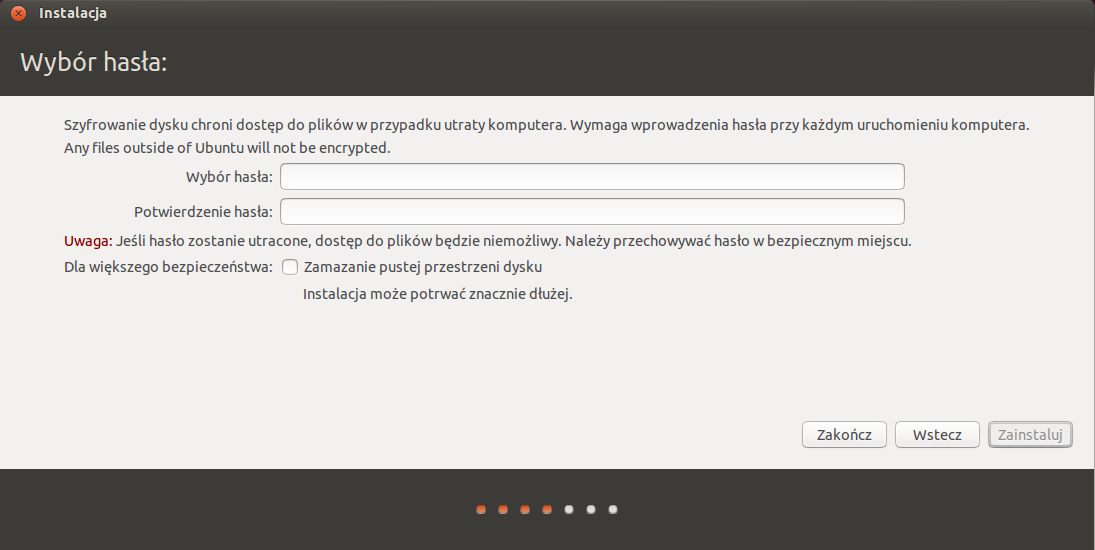
\includegraphics[scale=0.5]{images/instalator_partycjonowanie_szyfrowanie2.png}
\end{center}
Na tym ekranie podaj hasło - klucz do dysku twardego. To nie jest to samo hasło, które ustawisz dla swojego systemowego konta a jedynie hasło umożliwiające dostęp do danych zapisanych na dysku twardym. Pamiętaj, że jeżeli zapomnisz hasła jakie zostanie tu wprowadzone, nie będzie możliwości odzyskania zaszyfrowanych danych. Postaraj się też aby hasło nie było łatwe do odgadnięcia, ale łatwe dla ciebie do zapamiętania.

Opcja "Zamazanie pustej przestrzeni dysku" powoduje, że niewykorzystywana, wolna przestrzeń dysku zostanie nadpisana losowymi danymi. Taka operacja znacznie utródnia potencjalnym włamywaczą włamanie się do twoich danych. Miej na uwadze, że zamazywanie pustej przestrzeni może trwać bardzo długo, w zależności do tego ile miejsca przeznaczysz na Ubuntu.

\begin{flushright}
Kliknij na przycisk \textbf{Zainstaluj} aby przejść dalej.\\
Zostaniesz poproszony o potwierdzenie. Upewnij się, że wszystko jest w pożądku i kliknij \textbf{Naprzód}
W tym momencie wybrane zmiany zostaną zapisane na dysku twardym.\\
\end{flushright}
\clearpage

\subsection{Zaawansowane partycjonowanie}
\begin{center}
	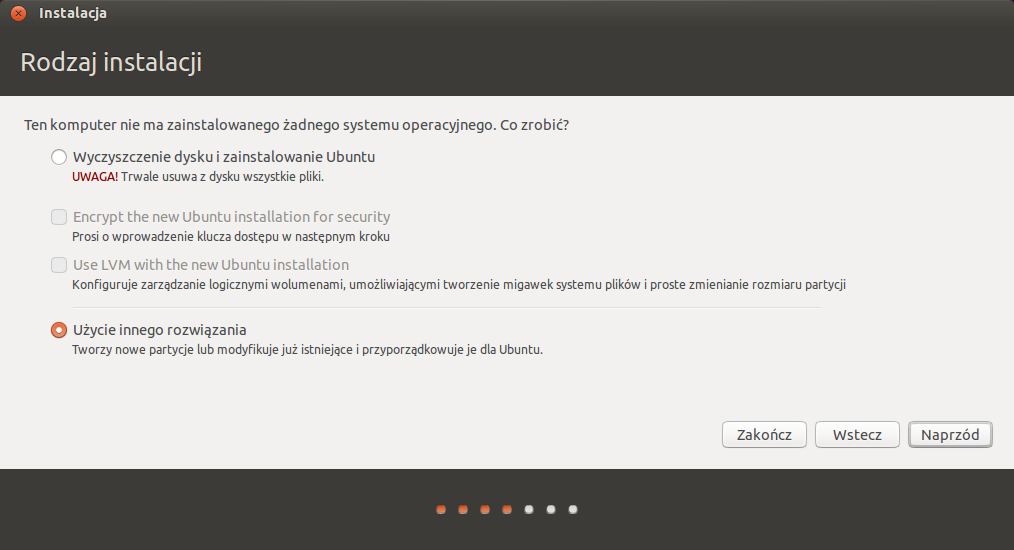
\includegraphics[scale=0.5]{images/instalator_partycjonowanie_gparted1.png}
\end{center}
"Użycie innego rozwiązania" uruchamia program GParted, który umożliwia nieograniczone modyfikowanie partycji na dysku twardym. Jest to opcja dla bardziej zaawansowanych użytkowników, którzy mają świadomość tego jak działa partycjonowanie i jak powinien zostac podzielony ich dysk twardy. Jednak jeżeli na swoim komputerze maasz zainstalowany więcej niż jeden system operacyjny lub z jakiegoś innego powodu przedstawione wcześniej opcje nie spełniają twoich wymagań, to konieczne będzie sięgnięcie do zaawansowanego partycjonowania.

Do GParted warto zajrzeć jeszcze z jednego powodu. Podział partycji stosowany przez automatyczną instalację nie jest idealny. Ręczne ustawienie partycji da większa kontrolę i pozwoli znacznie lepiej dopasować układ partycji.
\begin{flushright}
Kliknij na przycisk \textbf{Naprzód} aby przejść dalej.
\end{flushright}
\clearpage
\subsubsection{Ile miejsca przeznaczyć na Ubuntu}
\label{subsubsec:ile_miejsca}
Wirtualny dysk twardy użyty w tym przewodniku ma tylko 26.8 gigabajta pojemności. Twój dysk twardy będzie miał zapewne kilkaset gigabatów (jeżeli nie kilka terabajtów) pojemności. Dlatego też liczby jkimi się tu posługujemy będą miały niewielkie przełożenie na sytuację na twoim komputerze. W tym miejscu powinieneś się jednak zastanowić ile miejscach chcesz przeznaczyć na Ubuntu.

Ogólnie rzecz ujmując sprawa wygląda następująco
\begin{description}
\item[Partycja główna, root, /] - 6,2 Gigabajta to apsolutne minimum. 10 gigabajtów da pewną elastyczność i pozwoli zainstalować więcej programów. Nie ma potrzeby przesadzać w drugą stronę i tworzyć zbyt dużej partycji głównej, gdyż wolna przestrzeń będzie niewykorzystana. 15-20 gigabajtów w zupełności wystarczy.
\item[Partycja wymiany, swap] - na tej partycji zapisywane są dane, które nie mieszczą się w pamięci operacyjnej. Tutaj też przechowywany jest obraz RAMu kiedy poddajesz komputer hibernacji. Jeżeli korzystasz z hibernacji to wielkość partycji swap powinna być conajmniej taka jak ilość pamięci operacyjnej twojego komputera. Jeżeli nie planujesz korzystać z hibernacji to możesz nie tworzyć partycji wymiany. Jednak zaleca się jej stworzenie, jeżeli masz mniej niż 2 gigabajty RAMu. W takim wypadku nawet jeżeli nie korzystasz z hibernacji to dobrze jest stworzyć niewielką (300 - 400 megabajtów) partycję swap.
\item[Partycha domowa, /home] - W katalogu /home przechowywane są prywatne pliki użytkownika: zawartość pulpitu, dokumenty, filmy, muzyka i ustawienia programów. Katalog domowy może znajdować się na głównej partycji (/, root) lub można go wydzieć. Dobrą praktyką jest wydzielenie takiej partycji, gdyż w razie reinstalacji systemu nie trzeba będzie jej kasować. Nadpisana pozostanie tylko partycja główna, zaś wszystkie prywatne dane pozostaną niezmienione. Wielkość tej partycji zależy tylko i wyłącznie od tego jak wiele miejsca chcesz na nią przeznaczyć i jak wiele rzeczy zamierzasz na niej trzymać. 
\end{description}
\clearpage
\subsubsection{Główne okno programu GParted}
\begin{center}
	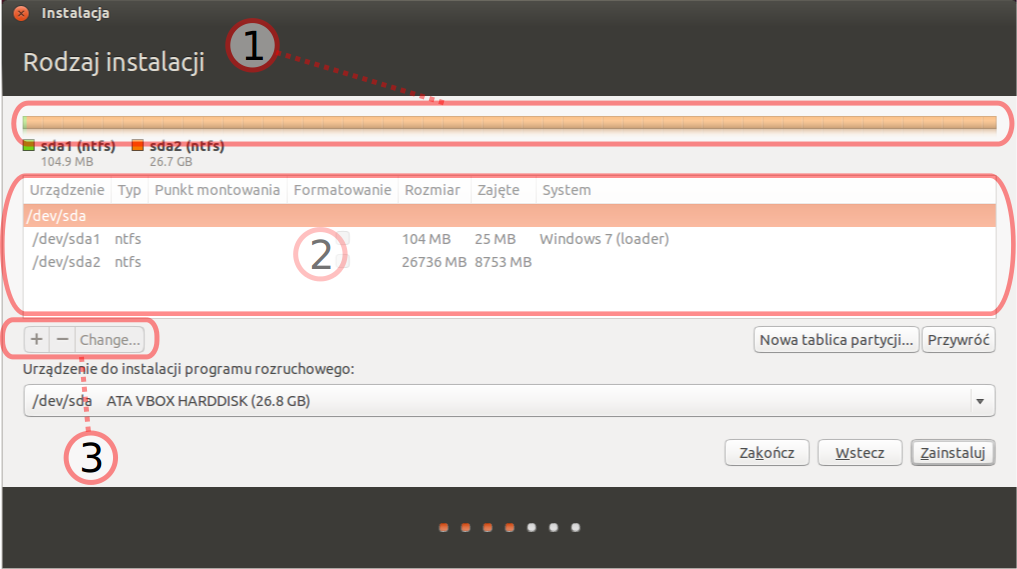
\includegraphics[scale=0.5]{images/instalator_partycjonowanie_gparted2.png}
\end{center}
Na powyższym obrazku widzisz głowne okno programu GParted. Wykryty został układ partycji na dysku twardym. Poziomy pasek (1) rozciągający się na całą szerokość okna jest graficzną reprezentacją układu partycji. Poniżej paska znajduje się legenda objaśnijaca użyte kolory. Tabela (2) znajdująca się w centralnej części okna przedstawia szczegółowe informacje na temat partycji na dysku twardym. Zestaw przycisków (3) służy do dodawania partycji(+), usówania partycji (-) lub ich modyfikacji(Change). Na chwilę obecną inne rzeczy nas nie interesują.

Powyższy układ dysków twardych oraz partycji jest tylko przykładem skonstruowanym na maszynie wirtualnej. Na Twoim komputerze liczby będą inne.

\clearpage
\begin{center}
	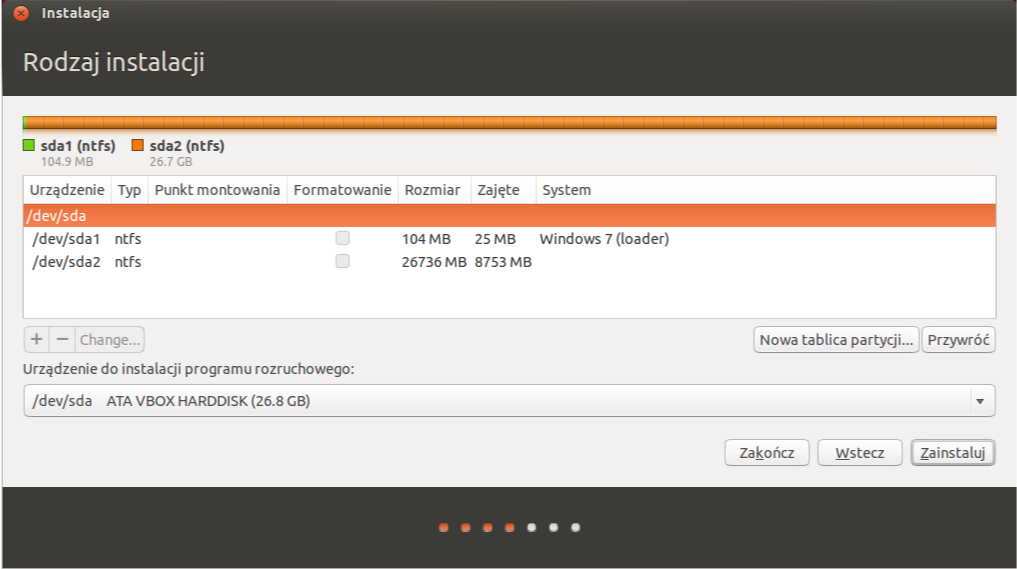
\includegraphics[scale=0.5]{images/instalator_partycjonowanie_gparted2_czysty.png}
\end{center}
Tabela umieszczona w centrum tego okna przedstawia informacje o poszczególnych partycjach obecnych na dysku twardym. Objaśnienie poszczególnych kolumn:
\begin{description}
\item[Urzadzenie] - Ścierzka do poszczególnych partycji na dysku twardym. Są to oznaczenia stosowane w systemach Unikoswych, do których należy Linux a więc i Ubuntu i opisują jak rozpoznawane są poszczególne partycje. W tym wypadku:
	\begin{description}
	\item[/dev/] - skrót od "Device", urządzenie
	\item[sda] - oznaczenie pierwszego dysktu twardego.
		\begin{description}
			\item[sd] - dysk na złączu SATA (sata disc)
			\item[a] - pierwszy dysk. Drugi dysk twardy miałby literę "b", trzeci "c" i tak dalej.
		\end{description}
	\item[sda1] - pierwsza partycja na pierwszym dysku twardym.
	\item[sda2] - druga partycja na pierwszym dysku twardym.
	\end{description}
\item[Typ] - rodzaj systemu plików. Sposób w jaki partycja została sformatowana. System Windows korzysta z ntfs, Ubuntu może korzystać z różnych.
\item[Punkt montowania] - miejsce w którym dana partycja zostanie "zamontowana", katalog w którym będzie widoczna zawartość tej partycji.
\item[Formatowanie] - zaznaczając to pole informujesz instalator, że dana partycja ma zostać sformatowana. Oznacza to utratę wszystkich danych na niej zapisanych.
\item[rozmiar] - pojemność partycji w megabajtach.
\item[Zajęte] - ile miejsca zostało zajęte na tej partycji
\item[System] - system operacyjny zainstalowany na danej partycji. Nie zawsze da się rozpoznać zainstalowany system. Nie każda partycja musi mieć zainstalowany system operacyjny. 
\end{description}
\clearpage
\subsubsection{Zaawansowane partycjonowanie - Instalacja obok systemu Windows}
\begin{center}
	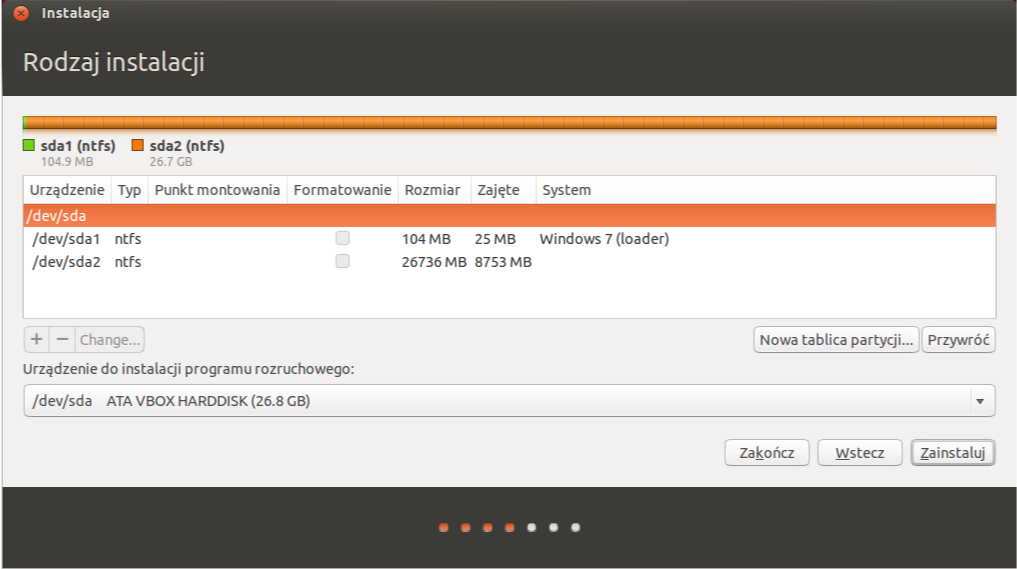
\includegraphics[scale=0.5]{images/instalator_partycjonowanie_gparted2_czysty.png}
\end{center}

Na powyższym obrazku widać dwie partycje utworzone przez instalator systemu Windows7. Partycja zielona o rozmiarze 104 megabajtów służy jako partycja dla programu rozruchowego systemu Windows. Duża, pomarańczowa partycja (26736 megabajtów) jest główna partycją systemu Windows7. Bardzo podobny układ partycji stosowany jest przez każdy z systemów z rodziny Windows.

Pierwszym krokiem jest zrobienie miejsca dla systemu Ubuntu. Kliknij na partycję /dev/sda2. Następnie kliknij na przycisk "Change" znajdujący się pod tabelą.. W otwartym oknie możesz zmniejszyć rozmiar wybranej partycji.
\clearpage

\begin{wrapfigure}{R}{0.4\textwidth}
		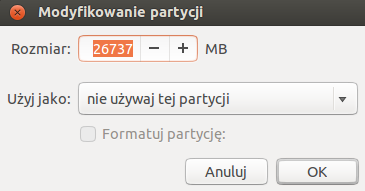
\includegraphics[scale=1]{images/instalator_partycjonowanie_gparted_zmniejszenie_partycji_windows.png}
\end{wrapfigure}
W polu Rozmiar podaj nowy rozmiar partycji. O tym ile miejsca potrzebujesz na Ubuntu przeczytasz w rozdziale \ref{subsubsec:ile_miejsca}: Ile miejsca przeznaczyć na Ubuntu. W polu podajesz rozmiar partycji w megabajtach. Jeden gigabajt to 1024 megabajty.\\
Upewnij się, że wybrano opcję "nie używaj tej partycji". Teraz kliknij przycisk \textbf{OK} a następnie \textbf{Naprzód} aby dokonać zmiany na partycji. Wykonanie żądanej zmiany może trwać dłuższą chwilę.

Na schemacie pojawiła się pusta, "dostępna przestrzeń" oznaczona kolorem szarym. Kliknij a nią, a następnie na przycisk (+) aby stworzyć nową partycję.
\begin{center}
	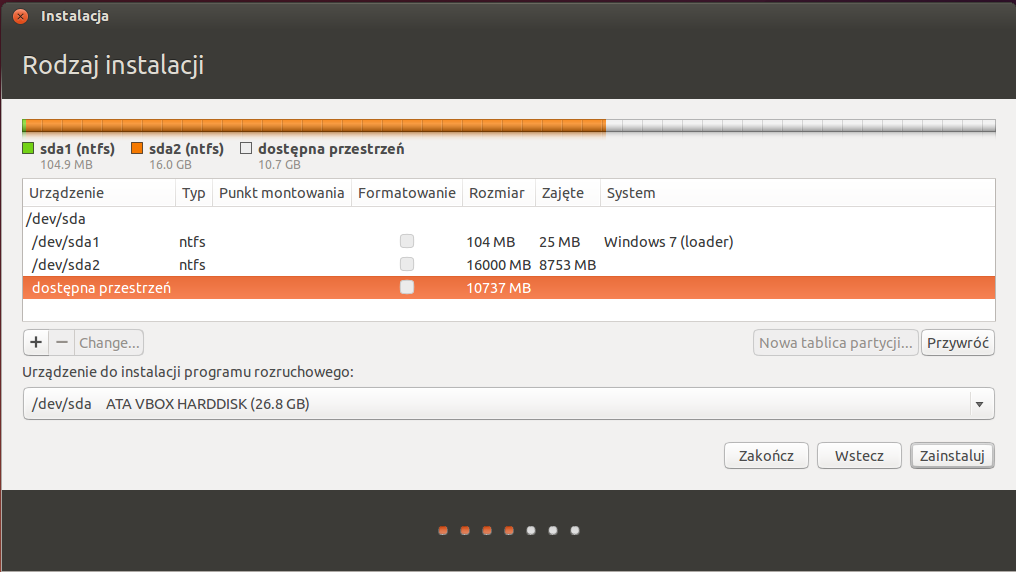
\includegraphics[scale=0.7]{images/instalator_partycjonowanie_gparted3.png}
\end{center}
\clearpage

\begin{wrapfigure}{R}{0.4\textwidth}
		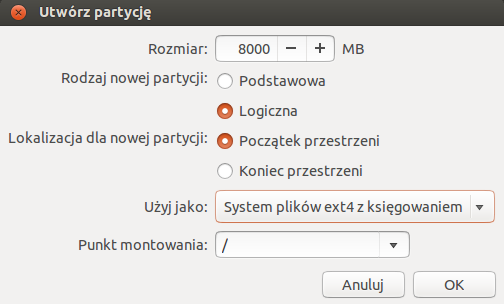
\includegraphics[scale=0.8]{images/instalator_partycjonowanie_gparted_dodaj_root.png}
\end{wrapfigure}
Po pierwsze musimy stworzyć partycję podstawową dla Ubuntu. O ilości miejsca potrzebnej na poszczególne partycje przeczytasz w sekcji \ref{subsubsec:ile_miejsca}: "Ile miejsca przeznaczyć na Ubuntu". Pozostałe opcje ustaw jak na rysunku.
\begin{description}
\item[Rozmiar] - rozmiar partycji w megabajtach
\item[Rodzaj nowej partycji] - jako, że system Windows korzysta z tablicy partycji ms-dos to jesteśmy ograniczeni do 4 partycji podstawowych. Aby nie było problemu, dla Ubuntu utworzymy partycje logiczne.
\item[Lokalizacja dla nowej partycji] - Czy partycja zostanie wyrównana do poczatku wolnej przestrzeni czy do jej końca. Nie ma to znaczenia dla działania systemu.
\item[Użyj jako] - jaki system plików ma być użyty do sformatowania tej partycji. Do wyboru jest wiele, ale w ramach tego przewodnika korzystamy z systemu ext4 z księgowaniem\footnote{Tematyka różnych systemów plików jest bardzo rozległa i z łatwością wypełniłaby kolejny Przewodnik.}
\item[Punkt montowania] - to nasza główna partycja, więc musi się znaleźdź na początku\footnote{W systemach Windows drzewo katalogów "zaczyna się" na "C:\\\\". W systemach Linuksowych zaczyna się na "/"}.
\end{description}
Kliknij na przycisk \textbf{OK} aby utworzyć nową partycję.
\clearpage
\begin{wrapfigure}{R}{0.4\textwidth}
		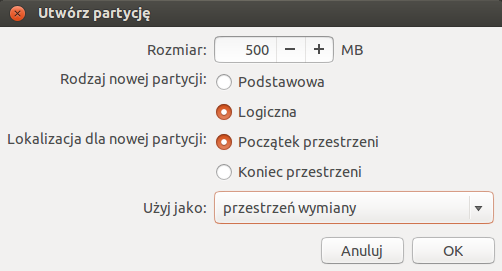
\includegraphics[scale=0.8]{images/instalator_partycjonowanie_gparted_dodaj_swap.png}
\end{wrapfigure}
Teraz utwórz partycję wymiany. Więcej o tej partycji przeczytasz w w sekcji \ref{subsubsec:ile_miejsca}: "Ile miejsca przeznaczyć na Ubuntu". Pozostałe opcje ustaw jak na rysunku. Kliknij na przycisk \textbf{OK} aby utworzyć nową partycję.

\begin{wrapfigure}{L}{0.4\textwidth}
		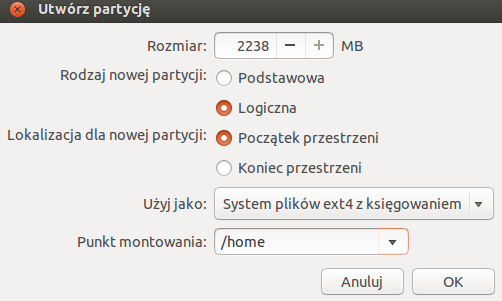
\includegraphics[scale=0.8]{images/instalator_partycjonowanie_gparted_dodaj_home.png}
\end{wrapfigure}
Na koniec pozostało utworzenie partycji domowej. Więcej o tej partycji przeczytasz w w sekcji \ref{subsubsec:ile_miejsca}: "Ile miejsca przeznaczyć na Ubuntu". Pozostałe opcje ustaw jak na rysunku. Kliknij na przycisk \textbf{OK} aby utworzyć nową partycję.
\clearpage

\begin{center}
	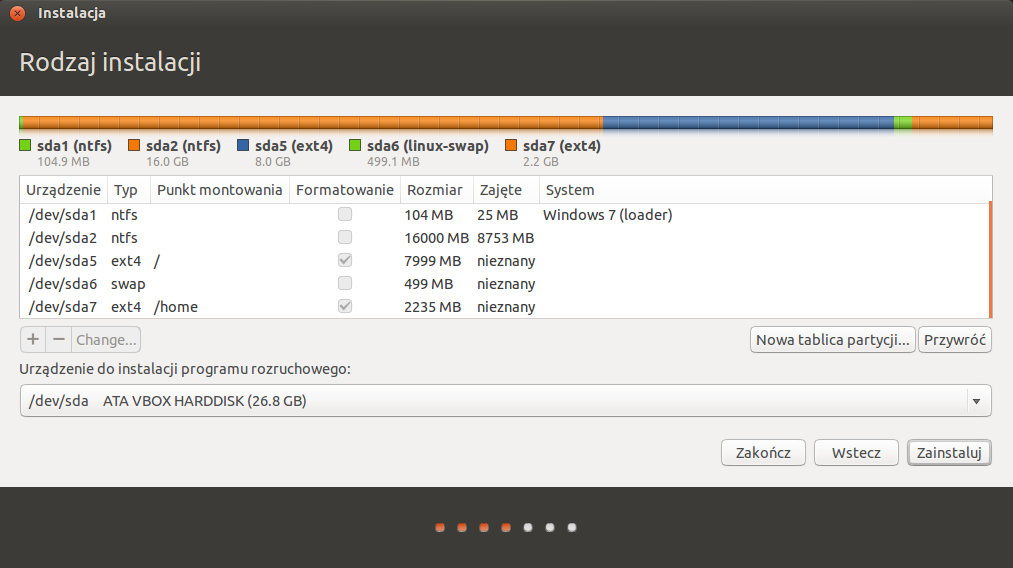
\includegraphics[scale=0.7]{images/instalator_partycjonowanie_gparted4.png}
\end{center}
Ekran programu GParted wygląda teraz mniej więcej tak jak na rysunku powyżej. Masz dwie partycje systemu Windows (ntfs), partycję wymiany systemu Linux (swap) oraz dwie partycje dla systemu Ubuntu (ext4). Upewnij się, że partycje ntfs \textbf{nie} są zaznaczone do sformatowania, zaś partycje ext4 tak. Kliknij na przycisk \textbf{Naprzód} aby wprowadzić zmiany na partycjach. Teraz możesz powrócić do lektury procesu instalacji w miejscu gdzie go przerwałeś.\\
Powrót do \ref{subsub:instalator_strefa_czasowa}: Wybór sterfy czasowej.